\documentclass[11pt]{article}
\usepackage[T1]{fontenc}
\usepackage[utf8]{inputenc}
\usepackage{enumerate}
\usepackage{setspace}
\usepackage{amsmath,amssymb,amsthm}
\usepackage{graphicx}
\usepackage{bbm}
\usepackage[round]{natbib}
\usepackage[nohead]{geometry}
\usepackage[bottom]{footmisc}
\usepackage{indentfirst}
\usepackage{endnotes}
\usepackage{graphicx}%
\usepackage{eurosym}
\usepackage{array}
\usepackage{booktabs}
\usepackage{caption}
\usepackage{subcaption}
\usepackage{rotating}
% \usepackage[hidelinks]{hyperref}
\usepackage{floatrow} %[capposition=top]
\floatsetup{footposition=bottom,capposition=top}
\renewcommand{\labelitemi}{--}
\renewcommand{\labelitemii}{$\bullet$}
\bibliographystyle{chicago}
% \geometry{left=1in,right=1in,top=1.00in,bottom=1.0in}
\let\olditemize\itemize
\renewcommand{\itemize}{
  \olditemize
  \setlength{\itemsep}{-1pt}
}

\begin{document}

\title{Competition between physician in Paris}
\author{Etienne Chamayou\thanks{e-mail:
\textit{etienne.chamayou@ensae.fr}}\medskip\\{\normalsize CREST and Department of Economics, Ecole Polytechnique }}
\maketitle

\sloppy%

\onehalfspacing

\textbf{Abstract:}

This note compares the locations and prices of general practitioners and ophthalmologists in Paris. Prices of general practitioners are largely regulated, hence the only way to increase income for most of them is to increase the number of patients. Conversely, ophthalmologists are often free to set prices. They can thus increase revenue through higher fees, which gives them an incentive to settle in wealthier areas. The comparison of geographic distributions and prices suggests that they do so in a significant way. The location of general practitioners, on the other hand, does not appear to be determined by population income.

\strut

\pagebreak%
\doublespacing

\section{Introduction}

The lack of physicians is a prominent health policy issue in France. Among the various specialties, ophthalmology is one of the most affected. As a consequence, a high proportion of ophthalmologists can freely set prices. On the other hand, most general practitioners remained constrained to set fees determined by law. While the debate certainly belongs in the public sphere, the complexity of the regulation and the lack of data make it difficult to develop an informed opinion. A crucial question which most likely limits our ability to reform the system is the absence of consensus as to whether healthcare should be viewed as a market or not. Data studied in this note show that the density and prices of sector 2 physicians are closely correlated to revenue at the district level. Since most ophthalmologists are sector 2, the densities of ophthalmologists across districts exhibit large inequalities, as opposed to these of general practitioners.

\section{Data}

Data were collected from www.annuairesante.ameli.fr, a website operated by the French National Health service which is designed to foster access to healthcare. All physicians are listed on the website, and information is provided regarding their fees.

\section{General Practitioners}

Except for one outlier, the number of GPs per inhabitants is relatively stable across Paris district. This remains true if one considers only sector 1 GPs (standard fees). Conversely, the number of sector 2 GPs per inhabitants increases with the district median fiscal revenue. The same pattern can be observed with the average consultation price per district.

\begin{figure}[H]
    \caption{Density of GPs vs. household revenue by district}
	\centering
		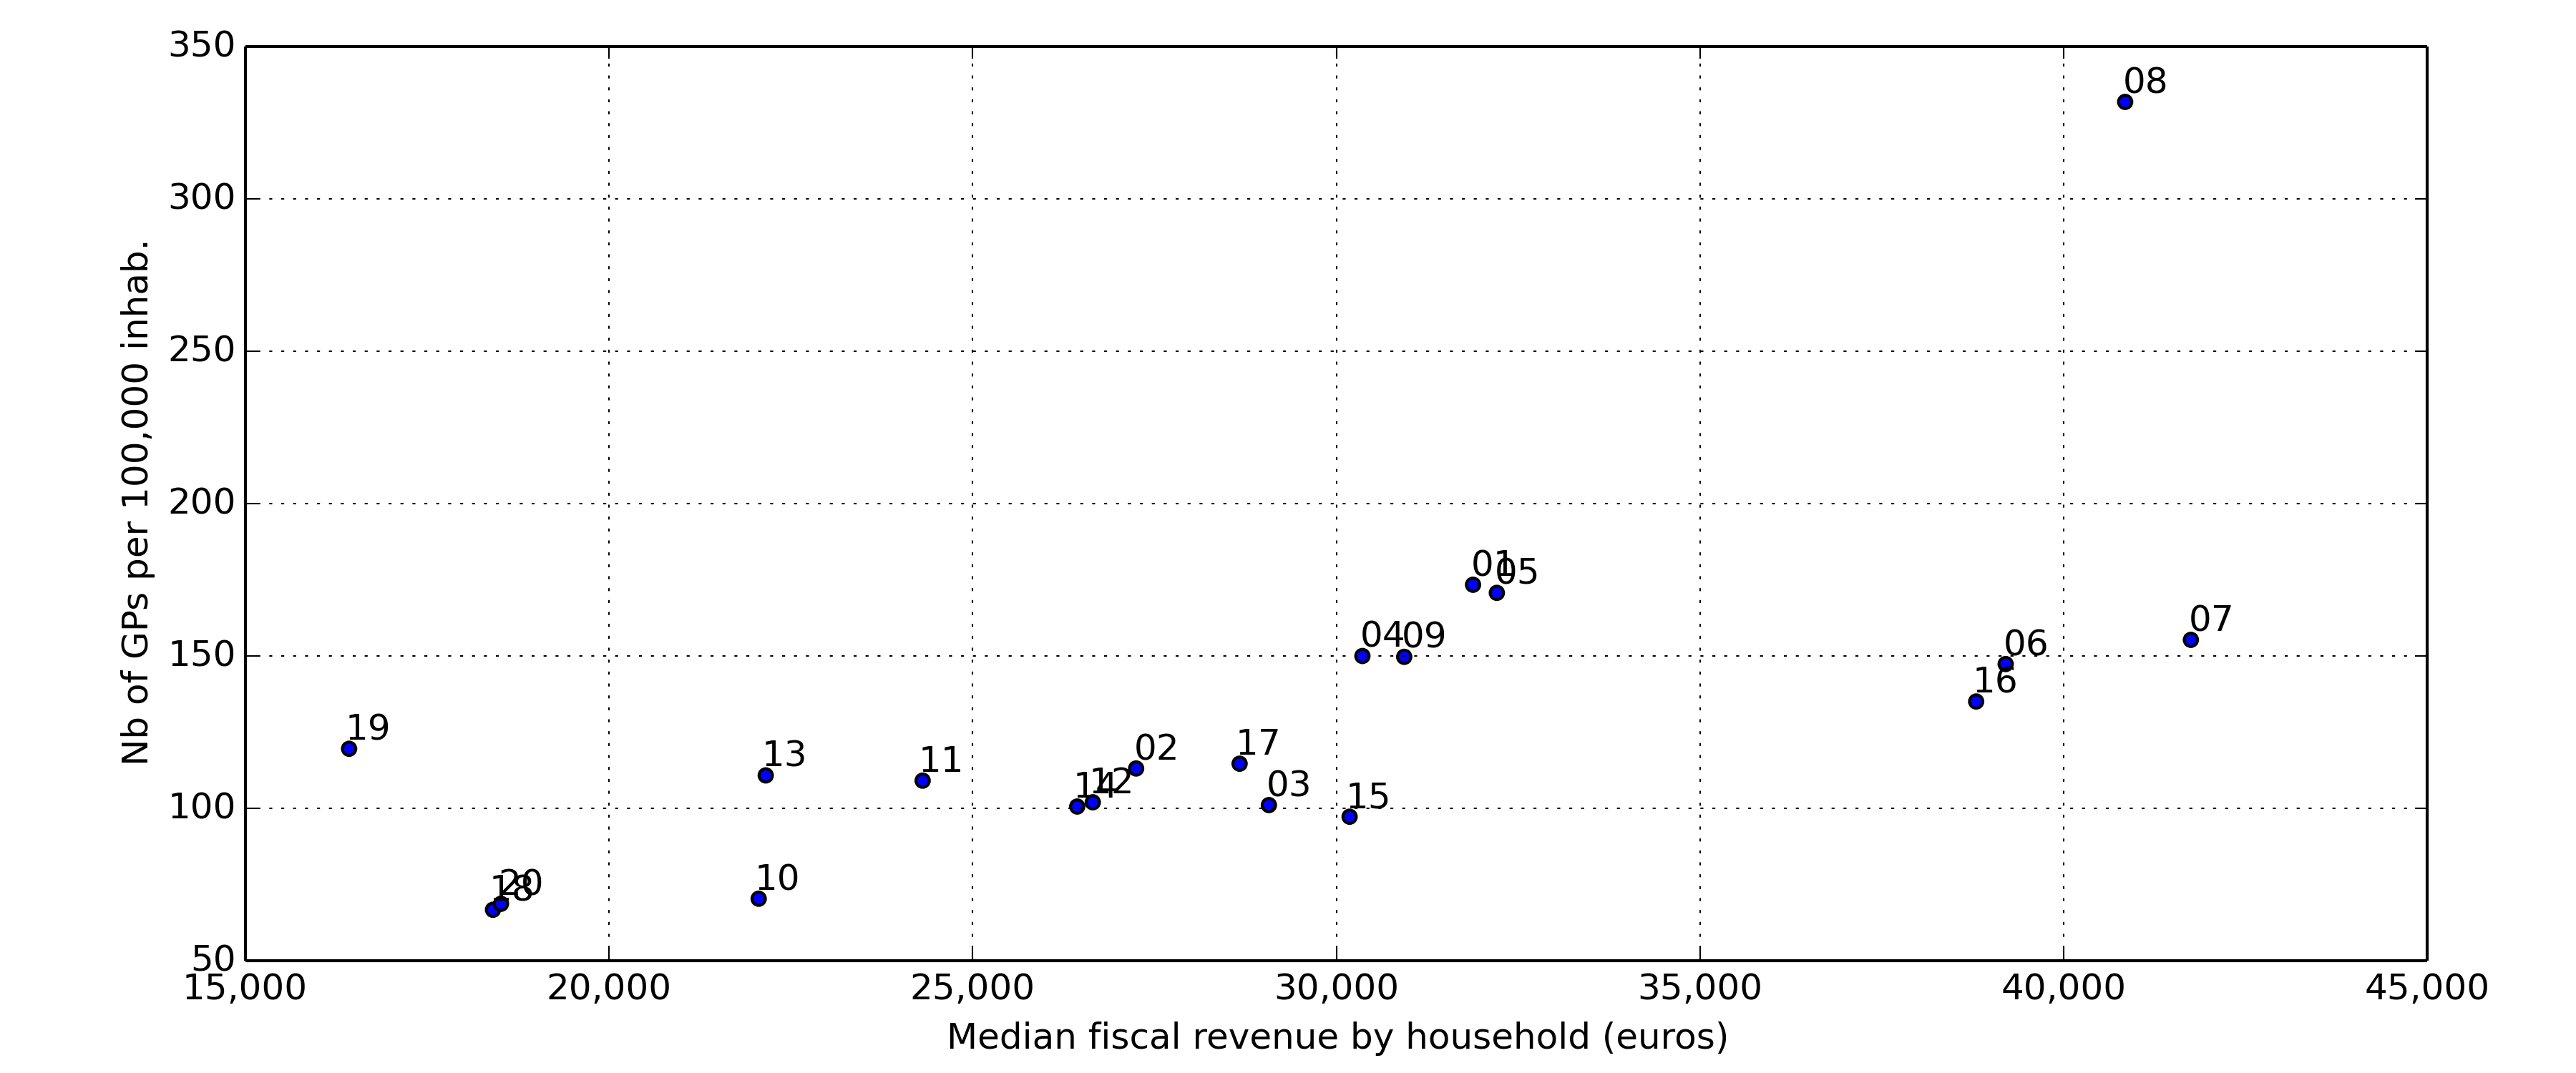
\includegraphics[width=16cm]{images/GP_Ardt_DensityVsRevenue.png}
\end{figure}

\begin{figure}[H]
    \caption{Density of sector 1 GPs vs. household revenue by district}
	\centering
		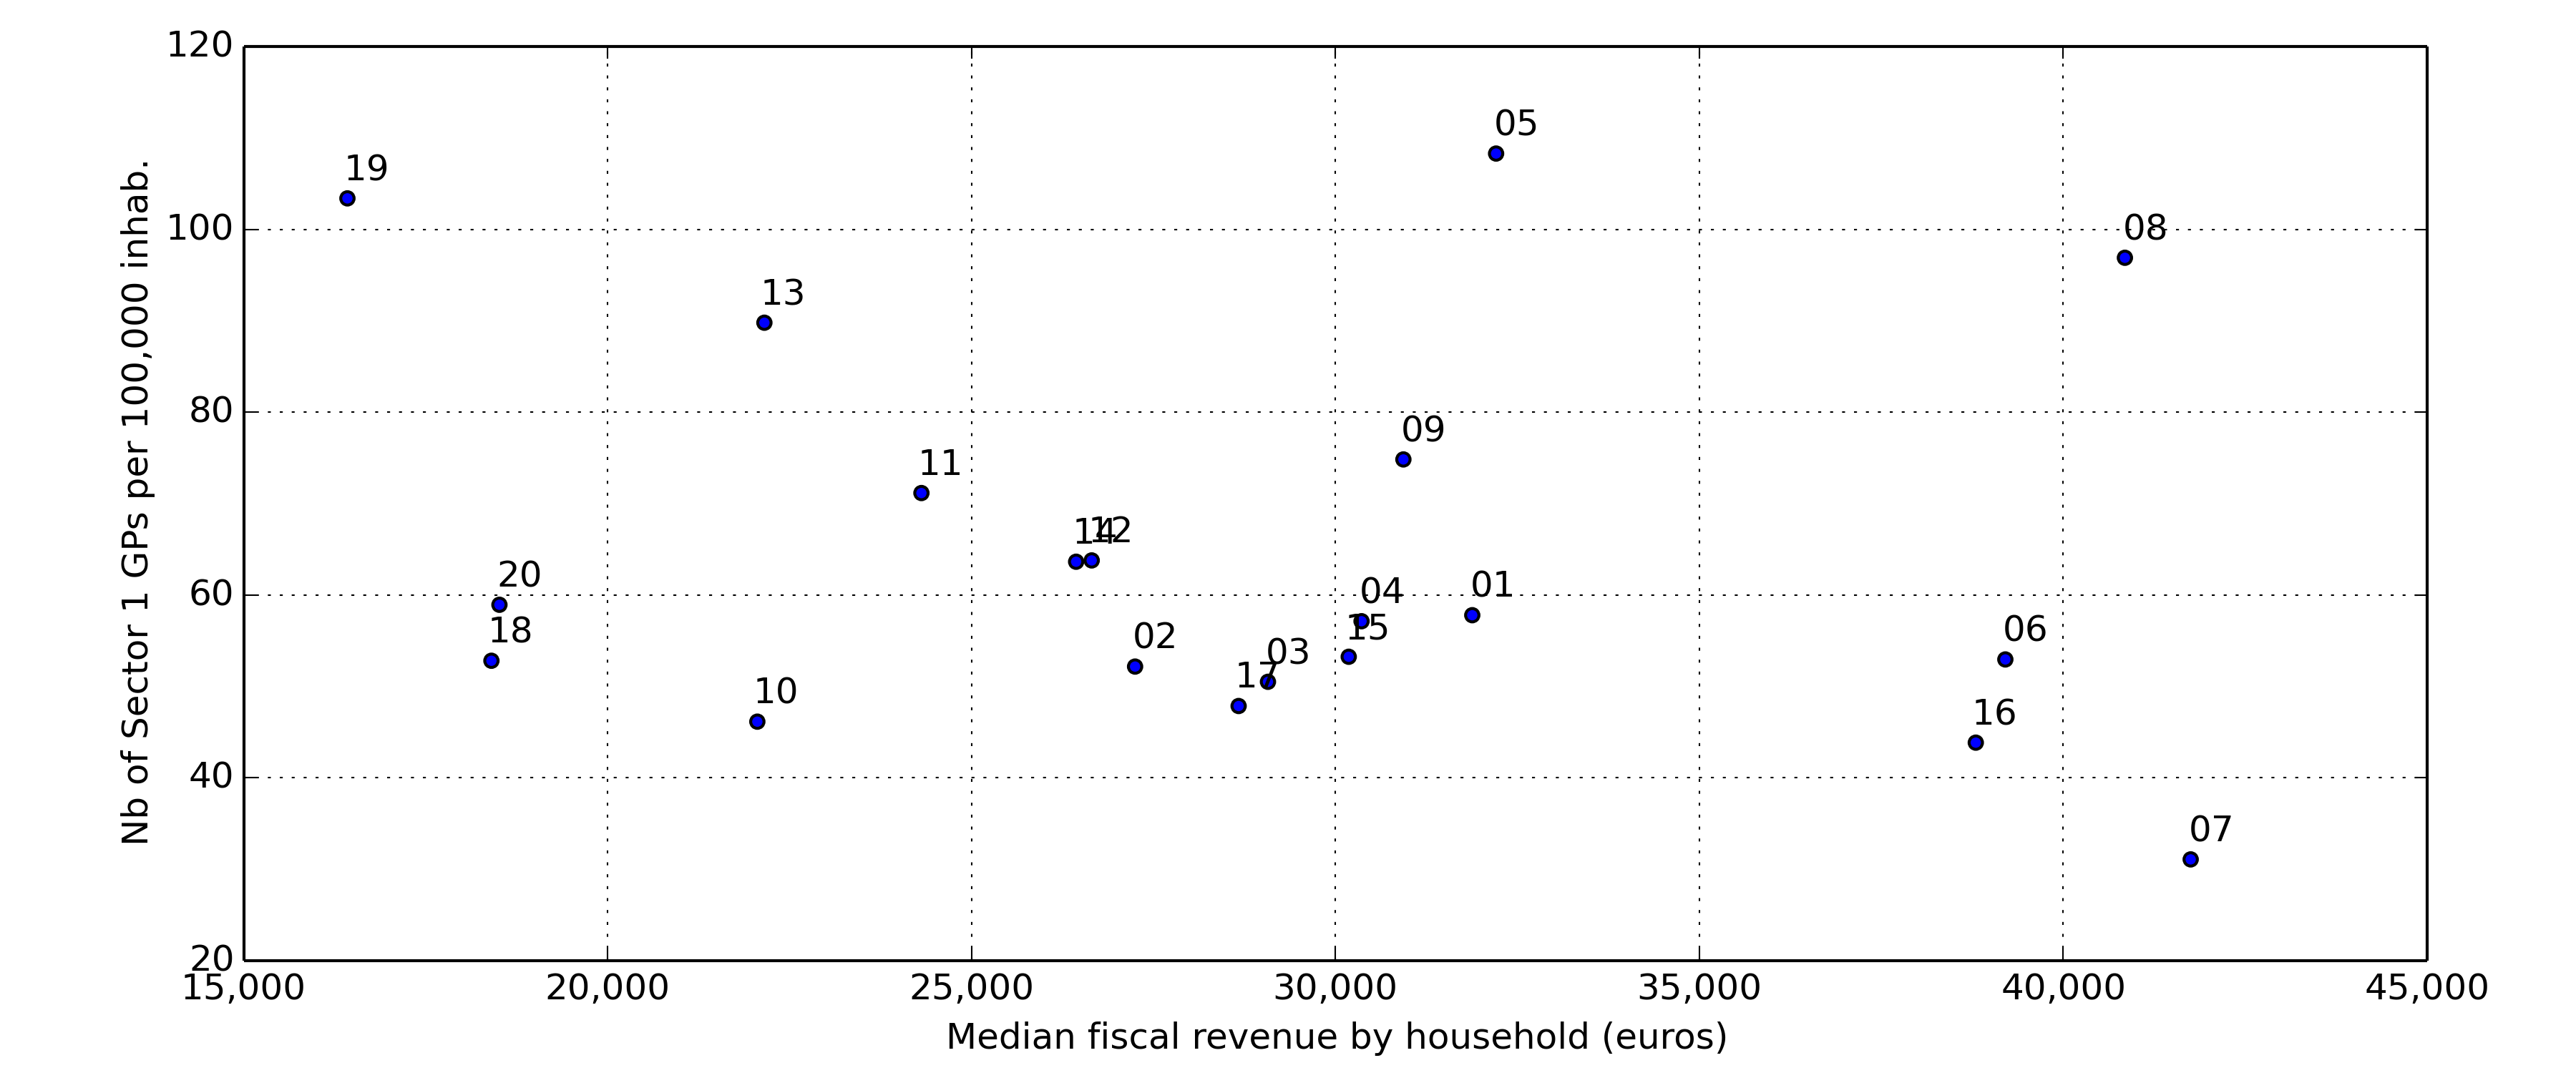
\includegraphics[width=16cm]{images/GP_Ardt_DensityS1VsRevenue.png}
\end{figure}

\begin{figure}[H]
    \caption{Density of sector 2 GPs vs. household revenue by district}
	\centering
		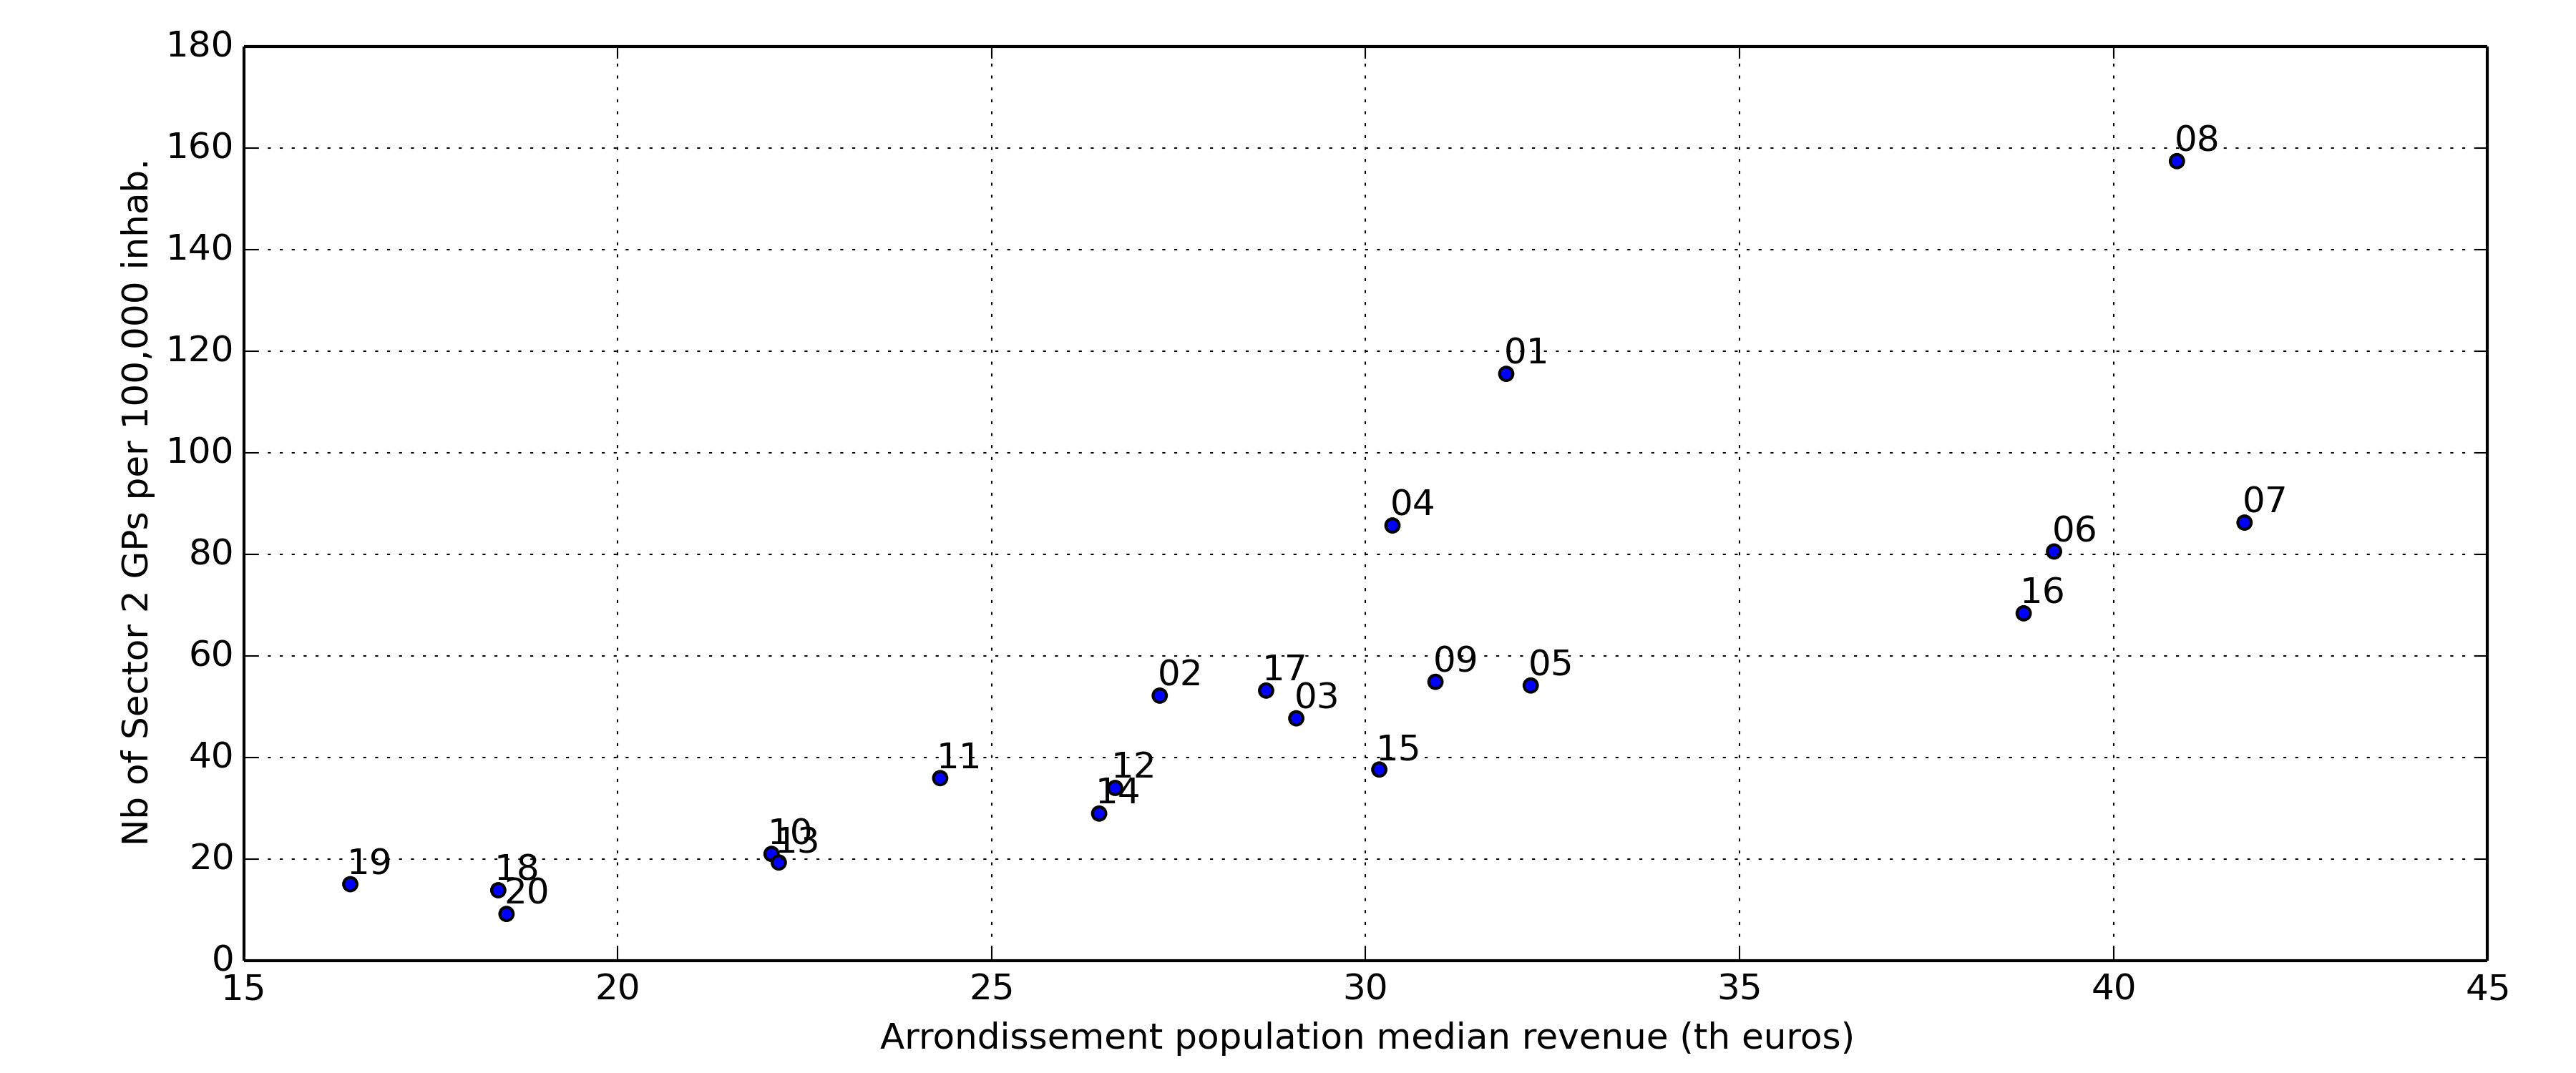
\includegraphics[width=16cm]{images/GP_Ardt_DensityS2VsRevenue.png}
\end{figure}

\begin{figure}[H]
    \caption{Average sector 2 GP consultation price vs. household revenue by district}
	\centering
		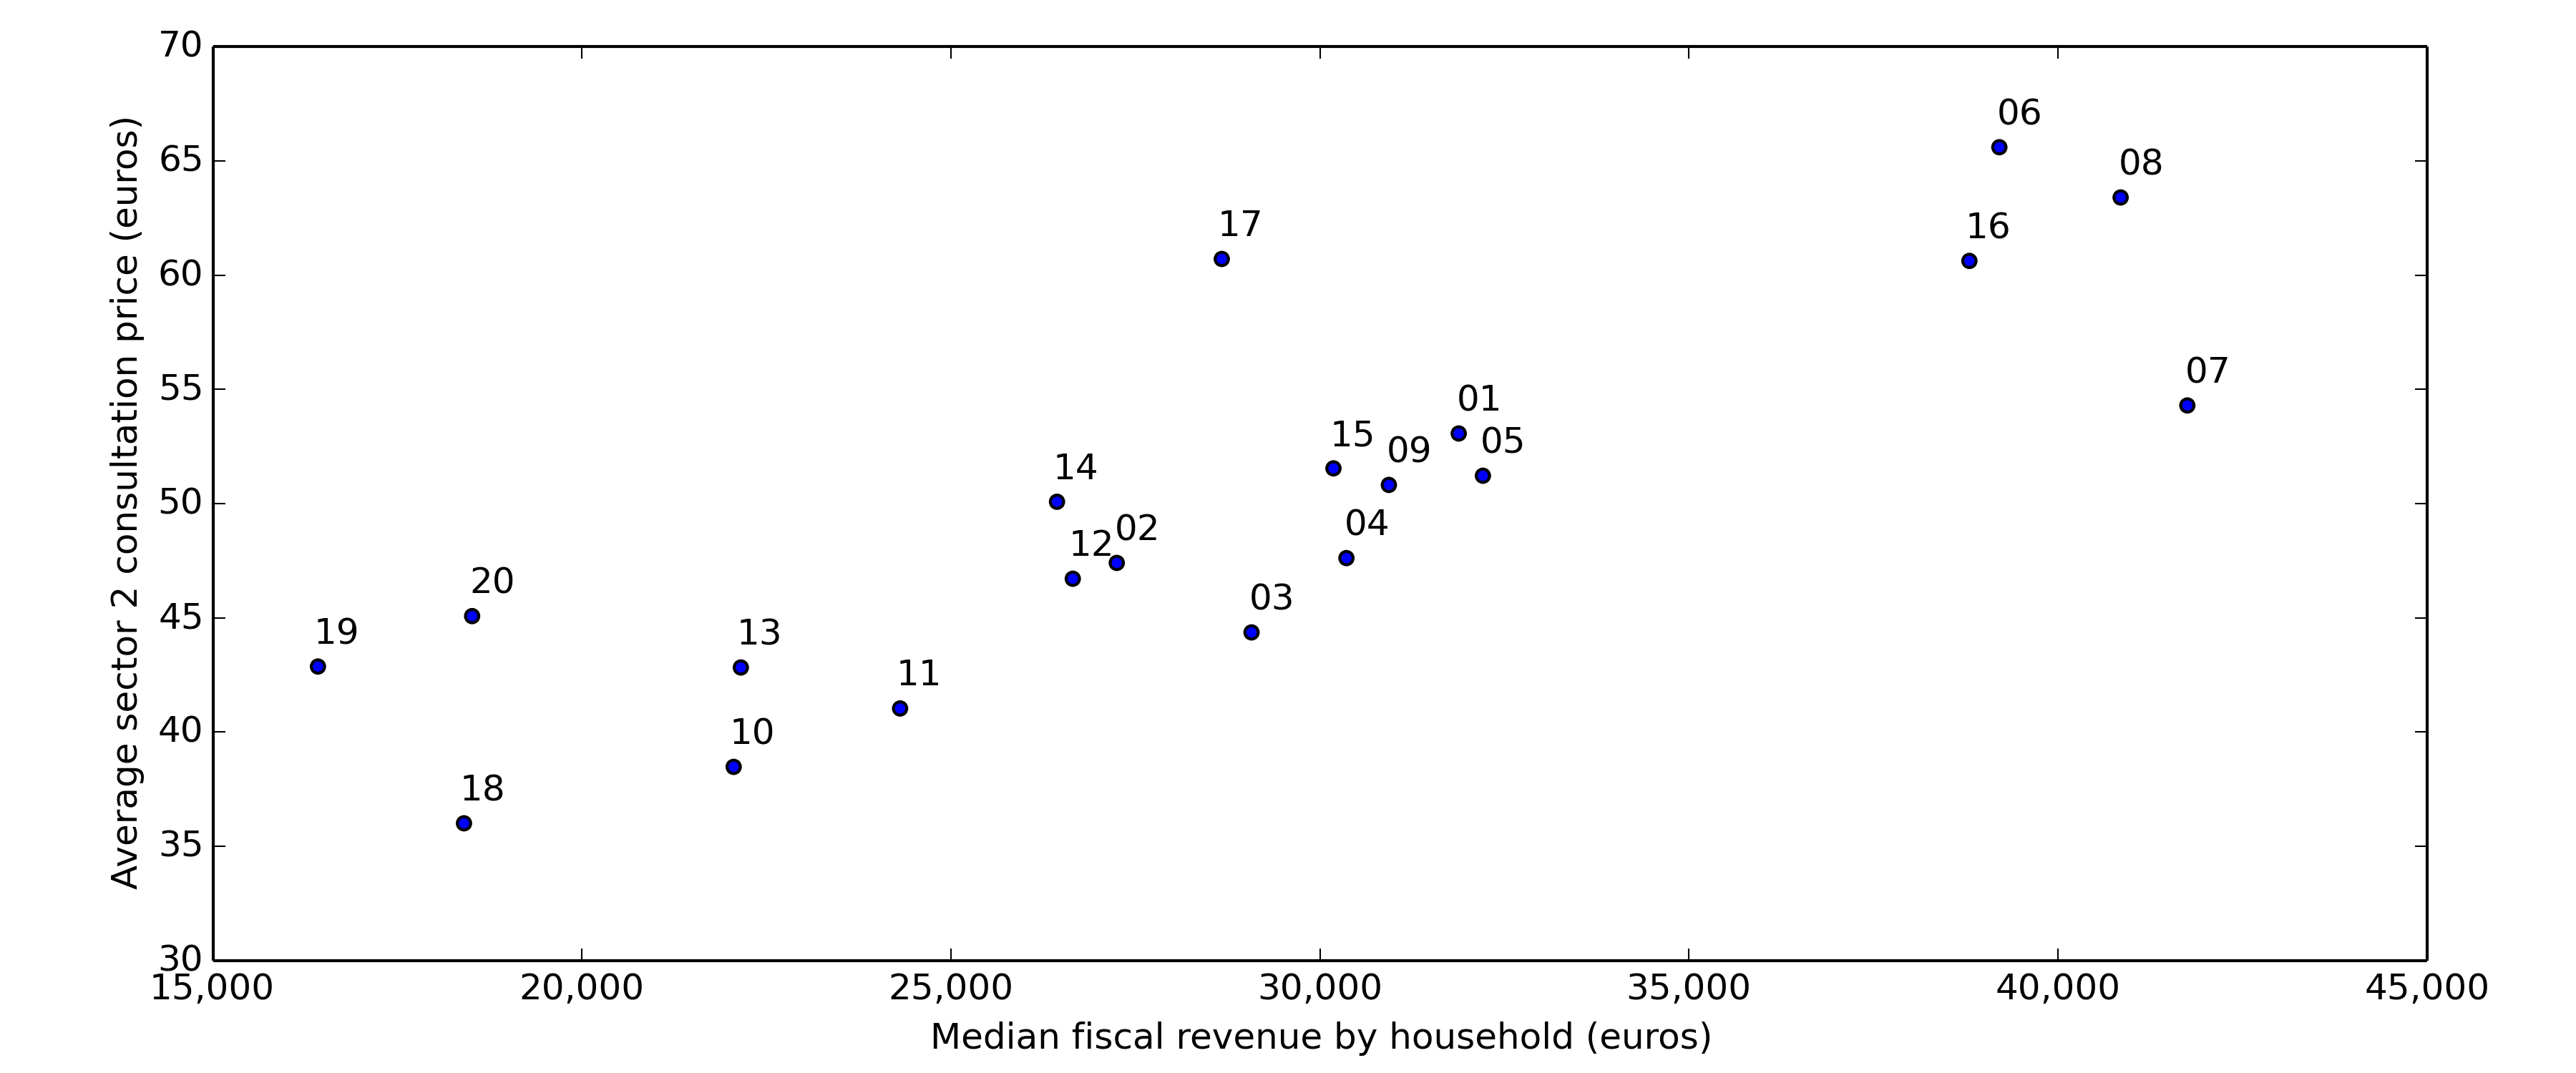
\includegraphics[width=16cm]{images/GP_Ardt_ConsultationS2VsRevenue.png}
\end{figure}

\section{Ophthalmologists}

The number of Ophthalmologists per inhabitants within appears to be much more determined by the district population revenue than in the case of GPs. The density of sector 1 ophthalmologists is relatively stable across districts, but these account for a small portion of ophthalmologists in Paris. Both the density of sector 2 ophthalmologists and their average consultation price appear to be largely correlated with revenue.

\begin{figure}[H]
    \caption{Density ophtalmologists vs. household revenue by district}
	\centering
		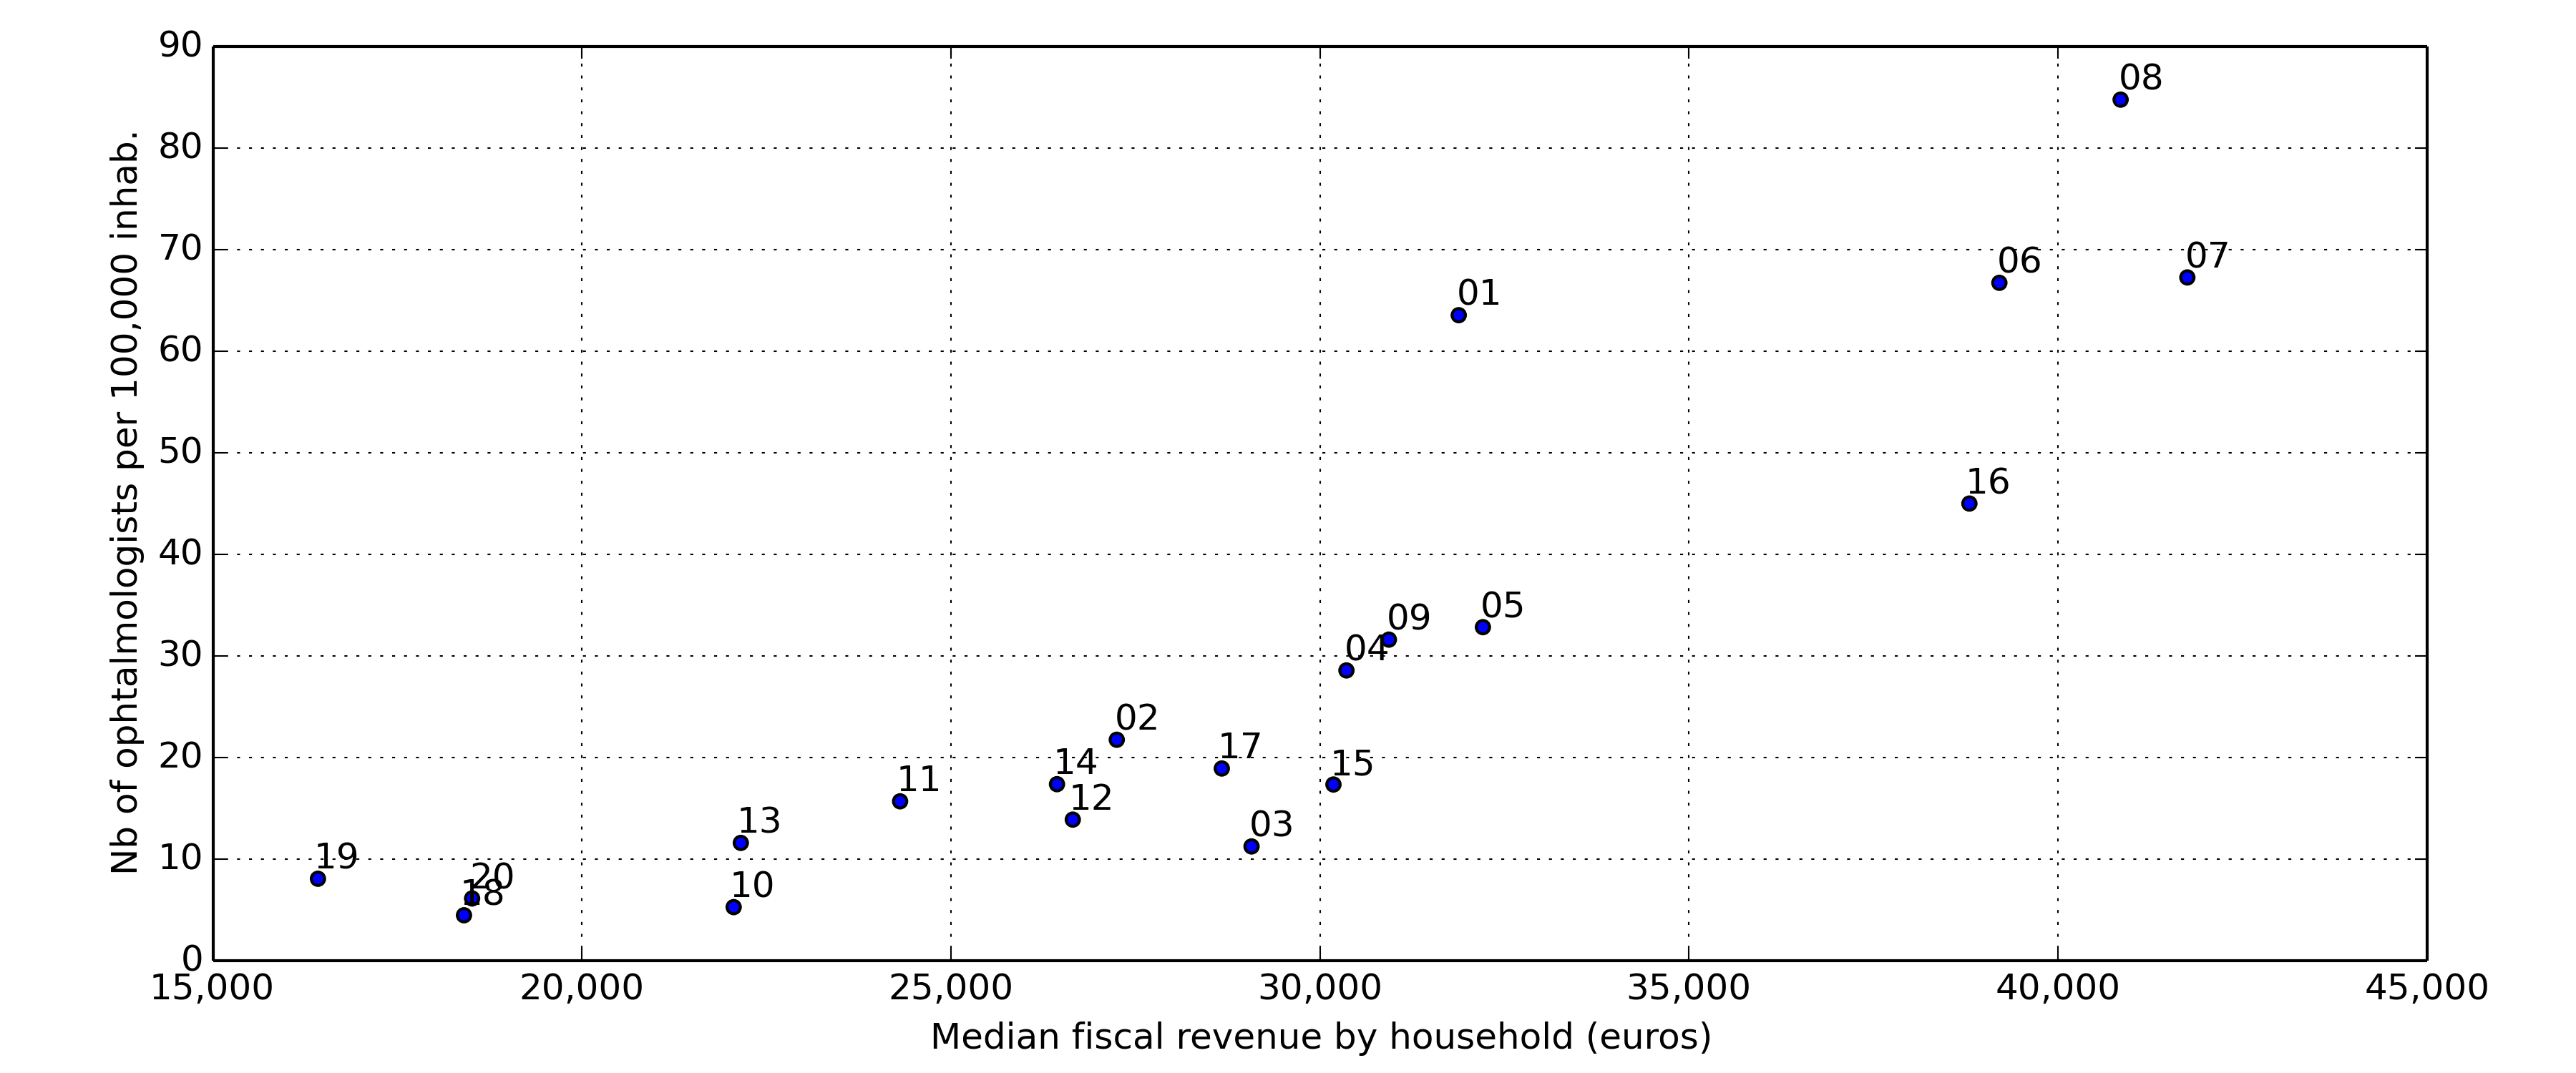
\includegraphics[width=16cm]{images/Ophtalmo_Ardt_DensityVsRevenue.png}
\end{figure}

\begin{figure}[H]
    \caption{Density of sector 1 ophtalmologists vs. household revenue by district}
	\centering
		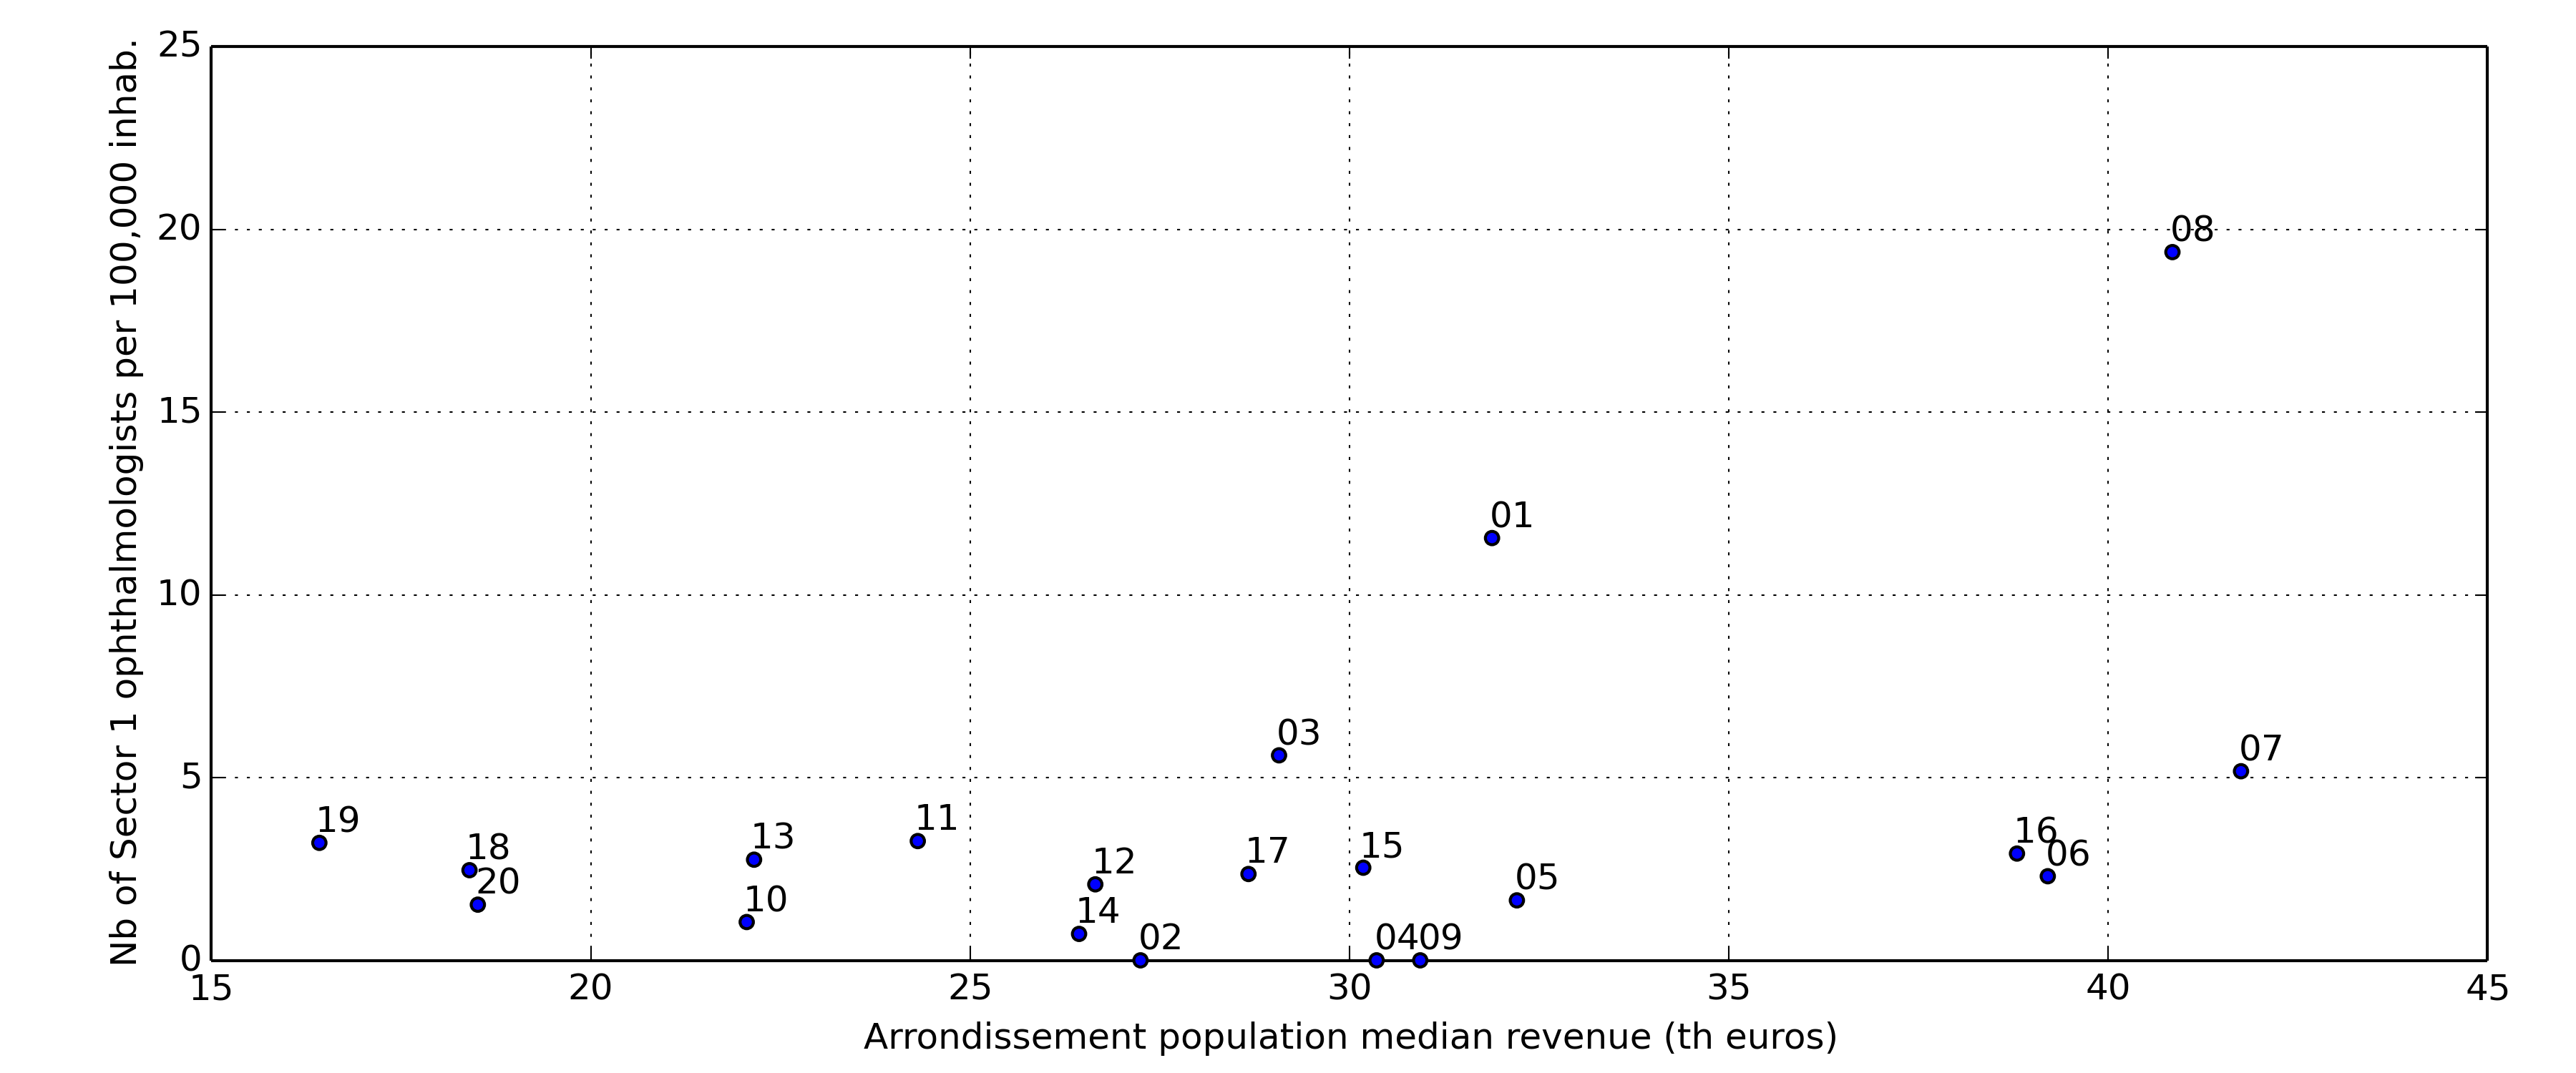
\includegraphics[width=16cm]{images/Ophtalmo_Ardt_DensityS1VsRevenue.png}
\end{figure}


\begin{figure}[H]
    \caption{Density of sector 2 ophtalmologists vs. household revenue by district}
	\centering
		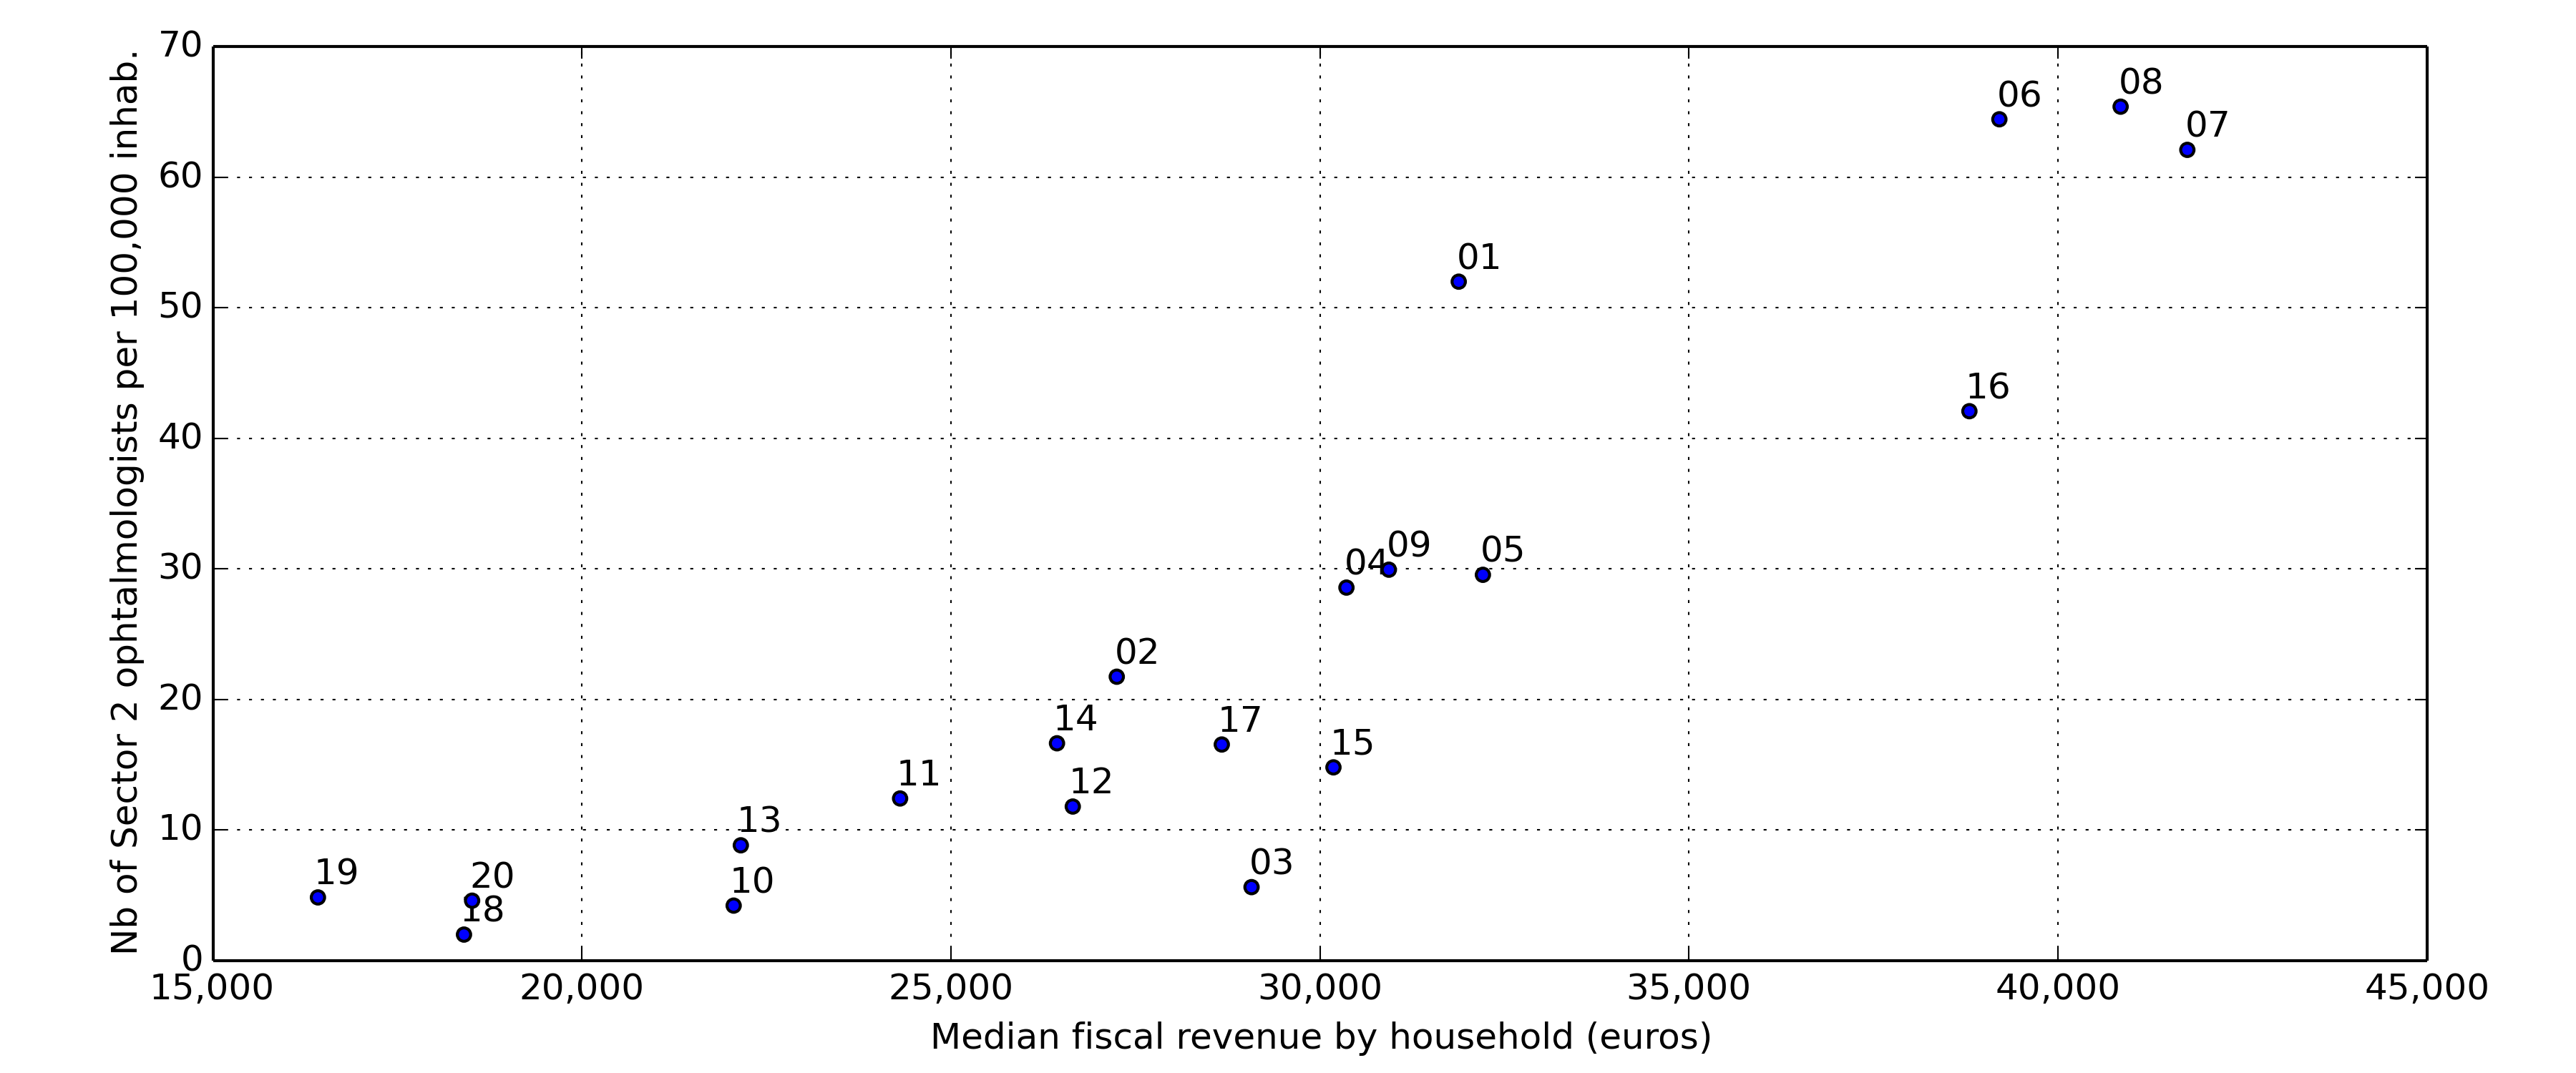
\includegraphics[width=16cm]{images/Ophtalmo_Ardt_DensityS2VsRevenue.png}
\end{figure}

\begin{figure}[H]
    \caption{Average sector 2 ophtalmologist consultation price vs. household revenue by district}
	\centering
		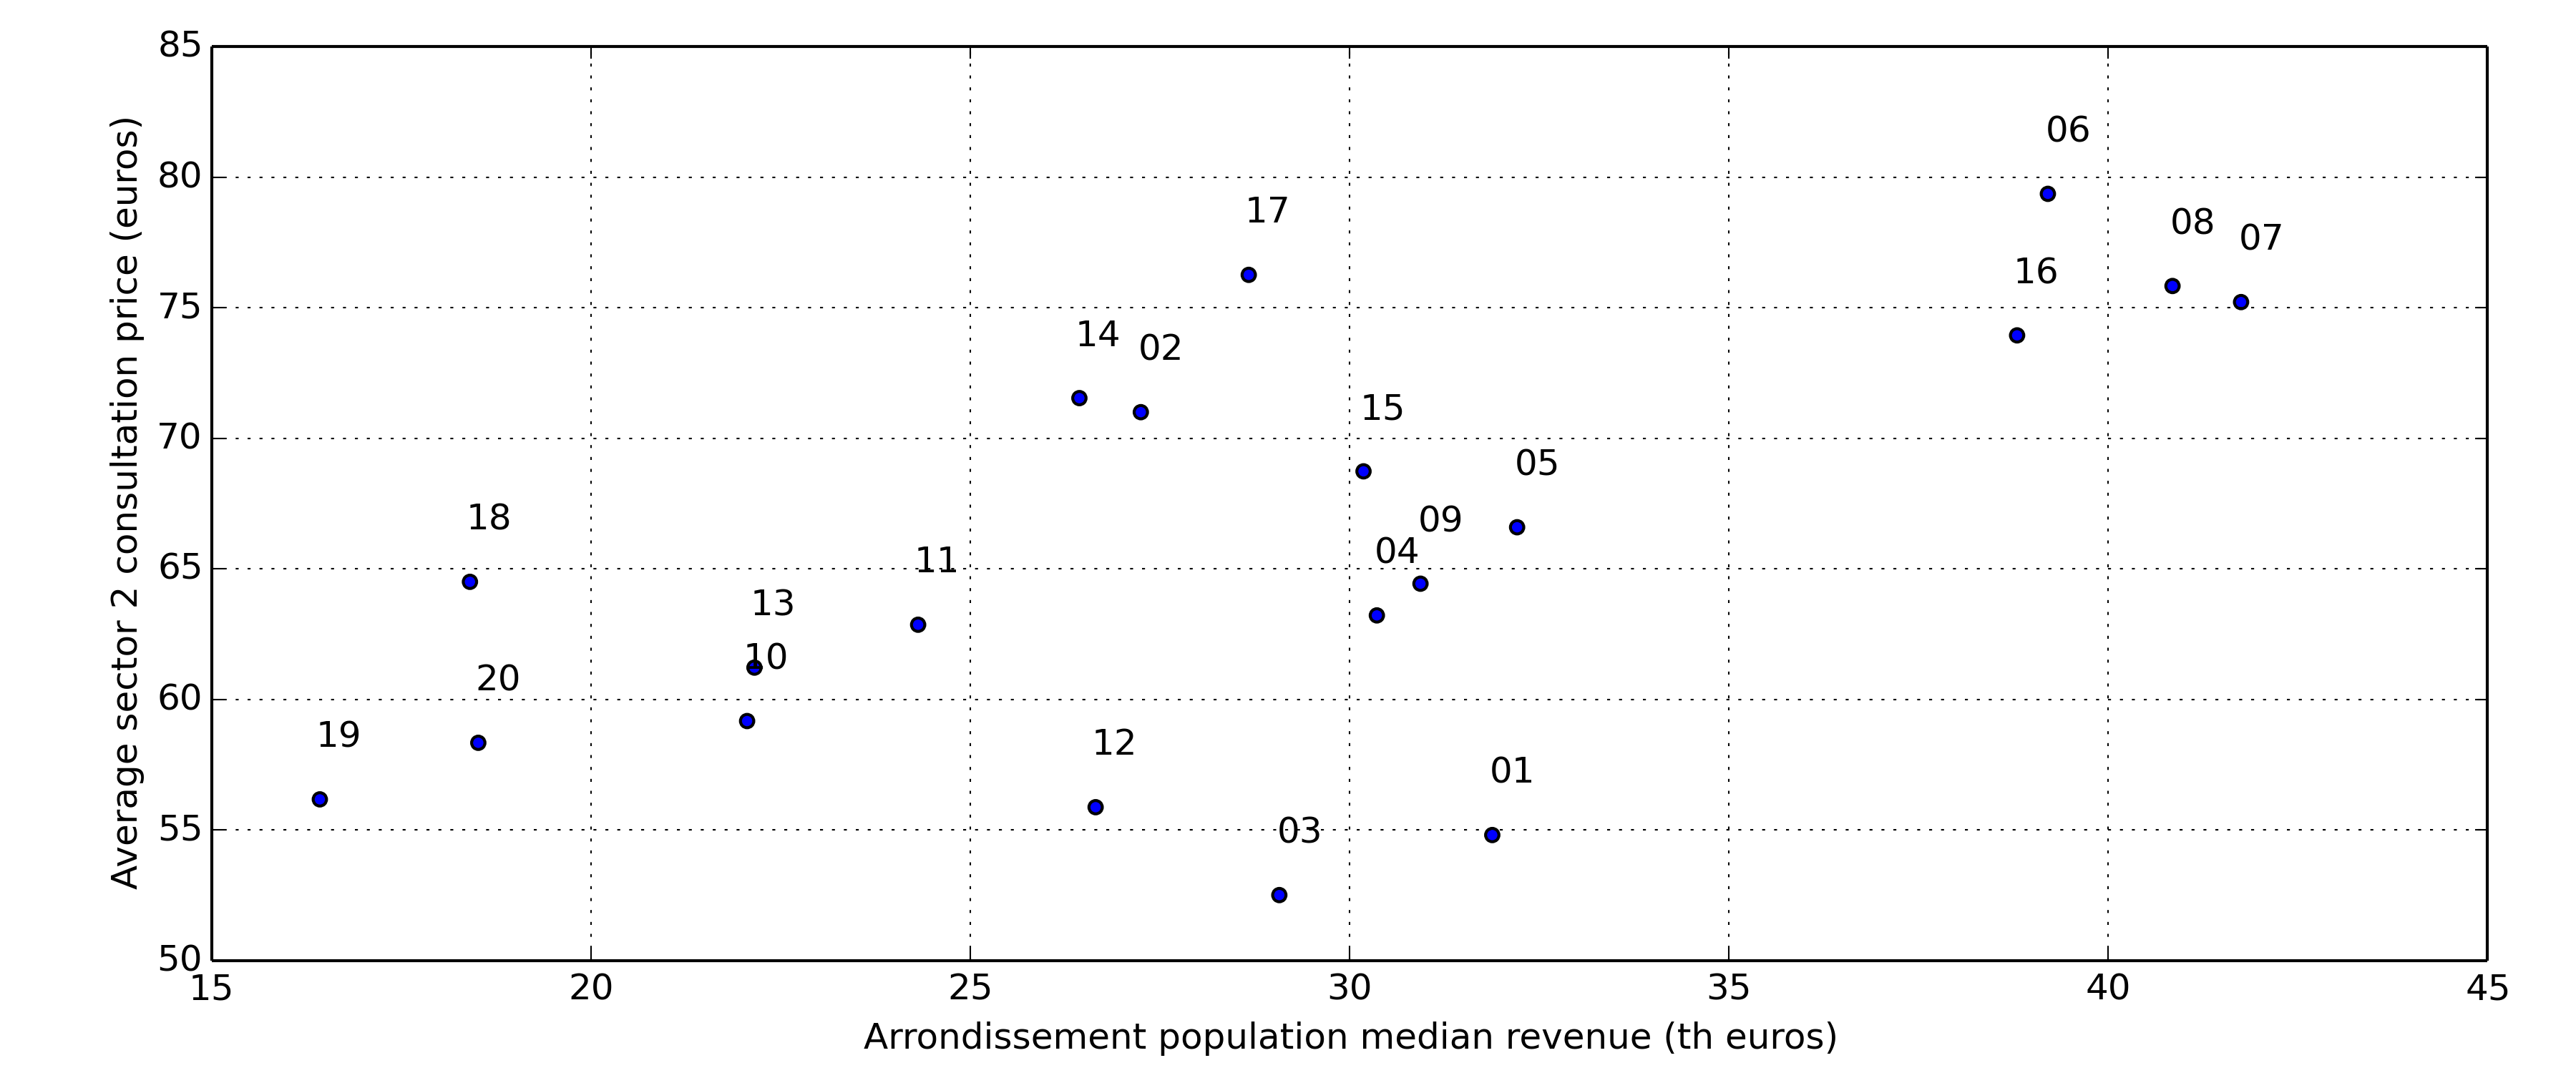
\includegraphics[width=16cm]{images/Ophtalmo_Ardt_ConsultationS2VsRevenue.png}
\end{figure}

\clearpage

\appendix


\end{document}
